\documentclass[aspectratio=169]{beamer}
\usetheme{Boadilla}
\usecolortheme{spruce}
\usepackage[utf8]{inputenc}
\usepackage[T1]{fontenc}
\usepackage{amsmath}
\usepackage{booktabs}
\usepackage{tikz}
\usetikzlibrary{arrows.meta, positioning, shapes.geometric}

% ── Metadata ──────────────────────────────────────────────────────────────────
\title{Lab Research Update}
\subtitle{Monthly Group Meeting}
\author{Dr.\ Wei Chen}
\institute{Computational Biology Lab}
\date{\today}

\begin{document}

\begin{frame}
  \maketitle
\end{frame}

\begin{frame}{Today's Agenda}
  \begin{enumerate}
    \item Project status update \hfill (5 min)
    \item New results \hfill (15 min)
    \item Discussion \hfill (10 min)
    \item Next steps \hfill (5 min)
  \end{enumerate}
\end{frame}

% ── Section 1 ─────────────────────────────────────────────────────────────────
\section{Project Status}

\begin{frame}{Where We Are}
  \begin{columns}
    \column{0.6\textwidth}
    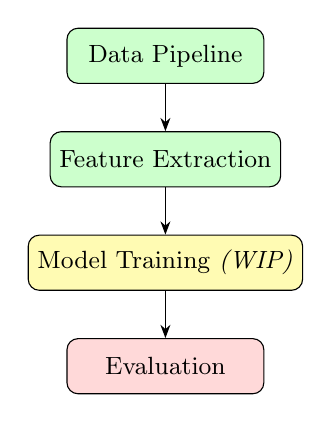
\begin{tikzpicture}[
      node distance=0.6cm and 2cm,
      box/.style={rectangle, draw, rounded corners, fill=green!20, minimum width=2.5cm, minimum height=0.7cm, font=\small},
      wip/.style={rectangle, draw, rounded corners, fill=yellow!30, minimum width=2.5cm, minimum height=0.7cm, font=\small},
      todo/.style={rectangle, draw, rounded corners, fill=red!15, minimum width=2.5cm, minimum height=0.7cm, font=\small},
    ]
      \node[box]  (a) {Data Pipeline};
      \node[box]  (b) [below=of a] {Feature Extraction};
      \node[wip]  (c) [below=of b] {Model Training \textit{(WIP)}};
      \node[todo] (d) [below=of c] {Evaluation};
      \draw[-{Stealth}] (a) -- (b);
      \draw[-{Stealth}] (b) -- (c);
      \draw[-{Stealth}] (c) -- (d);
    \end{tikzpicture}

    \column{0.35\textwidth}
    \textbf{Legend:}\\[0.3em]
    \textcolor{green!60!black}{\rule{0.8cm}{0.3cm}} Done \\[0.3em]
    \textcolor{yellow!70!black}{\rule{0.8cm}{0.3cm}} In Progress \\[0.3em]
    \textcolor{red!60!black}{\rule{0.8cm}{0.3cm}} TODO
  \end{columns}
\end{frame}

% ── Section 2 ─────────────────────────────────────────────────────────────────
\section{New Results}

\begin{frame}{Experiment: Ablation Study}
  \textbf{Question:} Which components contribute most to performance?

  \begin{table}
    \centering
    \begin{tabular}{lcc}
      \toprule
      \textbf{Configuration} & \textbf{AUROC} & \textbf{AP} \\
      \midrule
      Full model             & 0.921          & 0.887       \\
      w/o module A           & 0.891 (--3\%)  & 0.852       \\
      w/o module B           & 0.873 (--5\%)  & 0.831       \\
      w/o both               & 0.812 (--12\%) & 0.778       \\
      \bottomrule
    \end{tabular}
  \end{table}

  \begin{alertblock}{Finding}
    Module B is the most critical component — removing it causes a 5\% AUROC drop.
  \end{alertblock}
\end{frame}

\begin{frame}{Qualitative Analysis}
  \begin{itemize}
    \item \textbf{Case 1:} Model correctly identifies pattern X in 94\% of cases.
    \item \textbf{Case 2:} Failure mode — confuses Y with Z when context is limited.
    \item \textbf{Case 3:} Performance degrades on out-of-distribution samples.
  \end{itemize}

  \vspace{0.5em}
  \begin{block}{Insight}
    The model relies heavily on local context. Adding global attention resolves
    the failure mode in Case 2.
  \end{block}
\end{frame}

% ── Section 3 ─────────────────────────────────────────────────────────────────
\section{Discussion}

\begin{frame}{Open Questions}
  \begin{itemize}
    \item Should we increase dataset size or improve architecture?
    \item Is the observed variance due to random seed or data split?
    \item Collaboration opportunity with Group X?
  \end{itemize}

  \vspace{1em}
  \textbf{Action items from last meeting:}
  \begin{itemize}
    \item[\checkmark] Rerun experiment with fixed random seeds
    \item[\checkmark] Add data augmentation
    \item[$\square$] Write up results section of paper draft
  \end{itemize}
\end{frame}

% ── Section 4 ─────────────────────────────────────────────────────────────────
\section{Next Steps}

\begin{frame}{Timeline}
  \begin{description}
    \item[Week 1--2] Complete model training with final hyperparameters.
    \item[Week 3]    Evaluation on holdout test set. Internal paper draft.
    \item[Week 4]    Submit to conference (deadline: June 15).
    \item[Month 2]   Prepare rebuttal if needed. Extended journal version.
  \end{description}
\end{frame}

\begin{frame}[plain]
  \centering
  \vfill
  {\Large\bfseries Thanks for listening!}\\[1em]
  {\normalsize Feedback and suggestions welcome.}
  \vfill
\end{frame}

\end{document}
